\documentclass{../source/Experiment}

\major{信息工程}
\name{姚桂涛}
\title{喇叭天线的幅射特性测量及CST仿真}
\stuid{3190105597}
\college{信息与电子工程学院}
\date{\today}
\lab{东4-221}
\course{电磁场与电磁波}
\instructor{王子立}
\grades{}
\expname{喇叭天线的幅射特性测量及CST仿真}
\exptype{}
\partner{华天择}

\usepackage{caption}

\DeclareCaptionLabelSeparator{twospace}{\, }
\captionsetup{labelsep = twospace}

\begin{document}
    \makecover
    \makeheader

    \begin{center}
        \bfseries\Large{矩形波导馈电的角锥喇叭天线CST仿真}
    \end{center}
    \section{实验目的}
        \begin{enumerate}
            \item 了解并掌握波导喇叭天线的常用参数指标和分析方法.
            \item 了解熟悉CST软件的基本使用方法,学会运用其进行建模、仿真。
        \end{enumerate}
    \section{实验任务}
        用CST软件对特定的巨型波导喇叭天线进行建模、仿真,分析其辐射特性,并与喇叭天线辐射特性测量实验进行比较。
    \section{实验过程与结果}
        \subsection{模型建立}
            \subsubsection{建立工程}
                \begin{figure}[H]
                    \centering
                    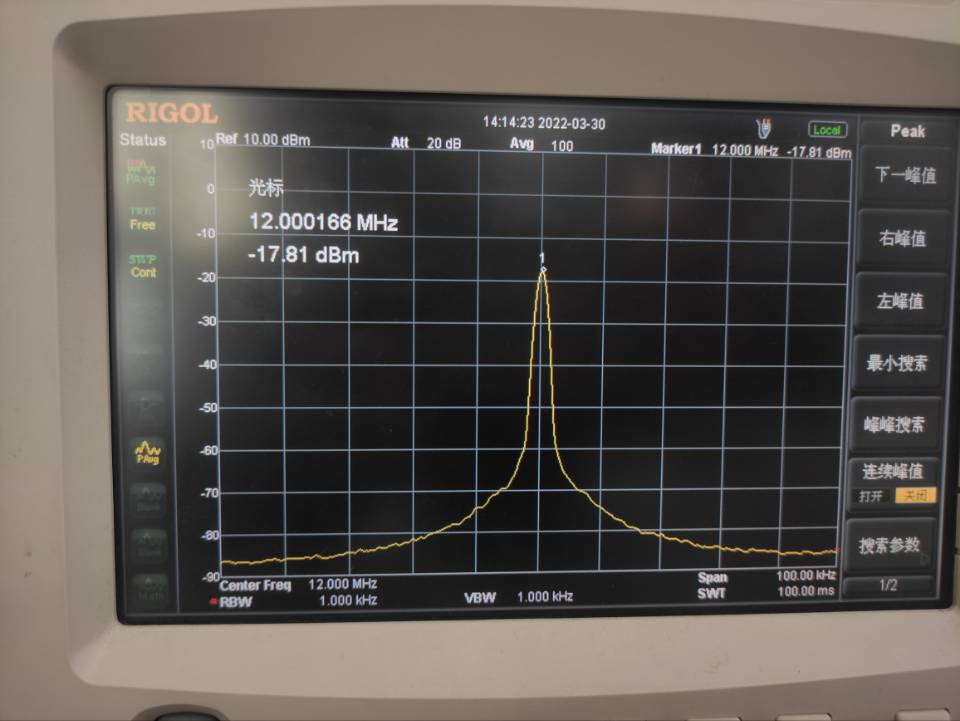
\includegraphics[width = 0.6\textwidth]{1}
                    \caption{}
                \end{figure}

                \begin{figure}[H]
                    \centering
                    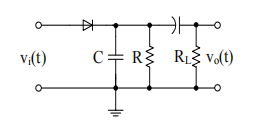
\includegraphics[width = 0.6\textwidth]{2}
                    \caption{}
                \end{figure}

            \subsubsection{参数设置}
                \begin{figure}[H]
                    \centering
                    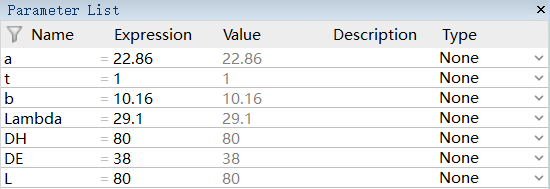
\includegraphics[width = 0.6\textwidth]{0}
                    \caption{}
                \end{figure}
            \subsubsection{创建矩形}

            \begin{figure}[H]
                \centering
                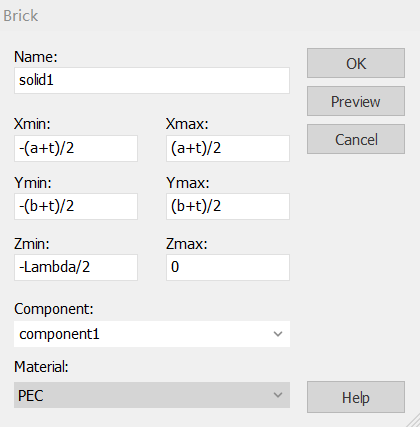
\includegraphics[width = 0.5\textwidth]{3}
                \caption{}
            \end{figure}
            
            \begin{figure}[H]
                \centering
                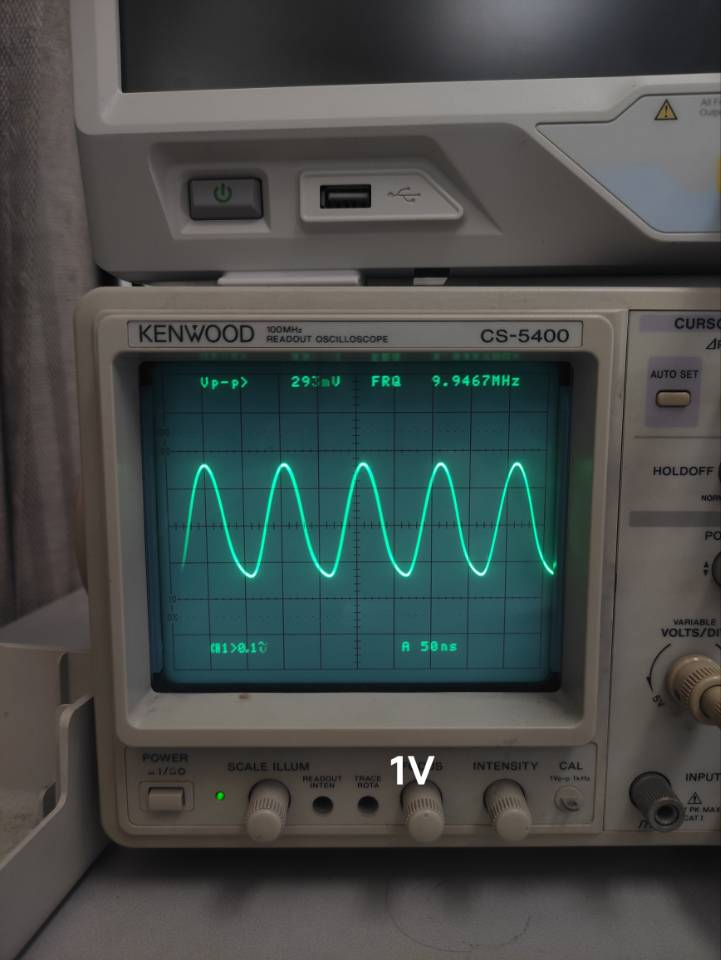
\includegraphics[width = 0.8\textwidth]{4}
                \caption{}
            \end{figure}
            
            \subsubsection{建立喇叭模型}

            建立喇叭口径面
            \begin{figure}[H]
                \centering
                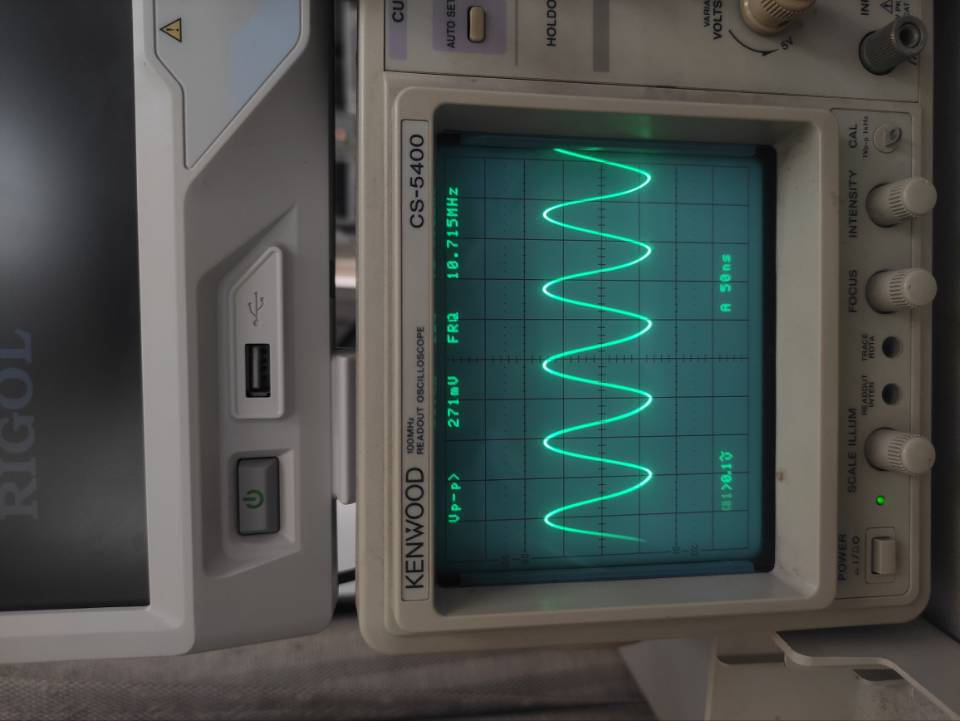
\includegraphics[width = 0.4\textwidth]{5}
                \caption{}
            \end{figure}

            \begin{figure}[H]
                \centering
                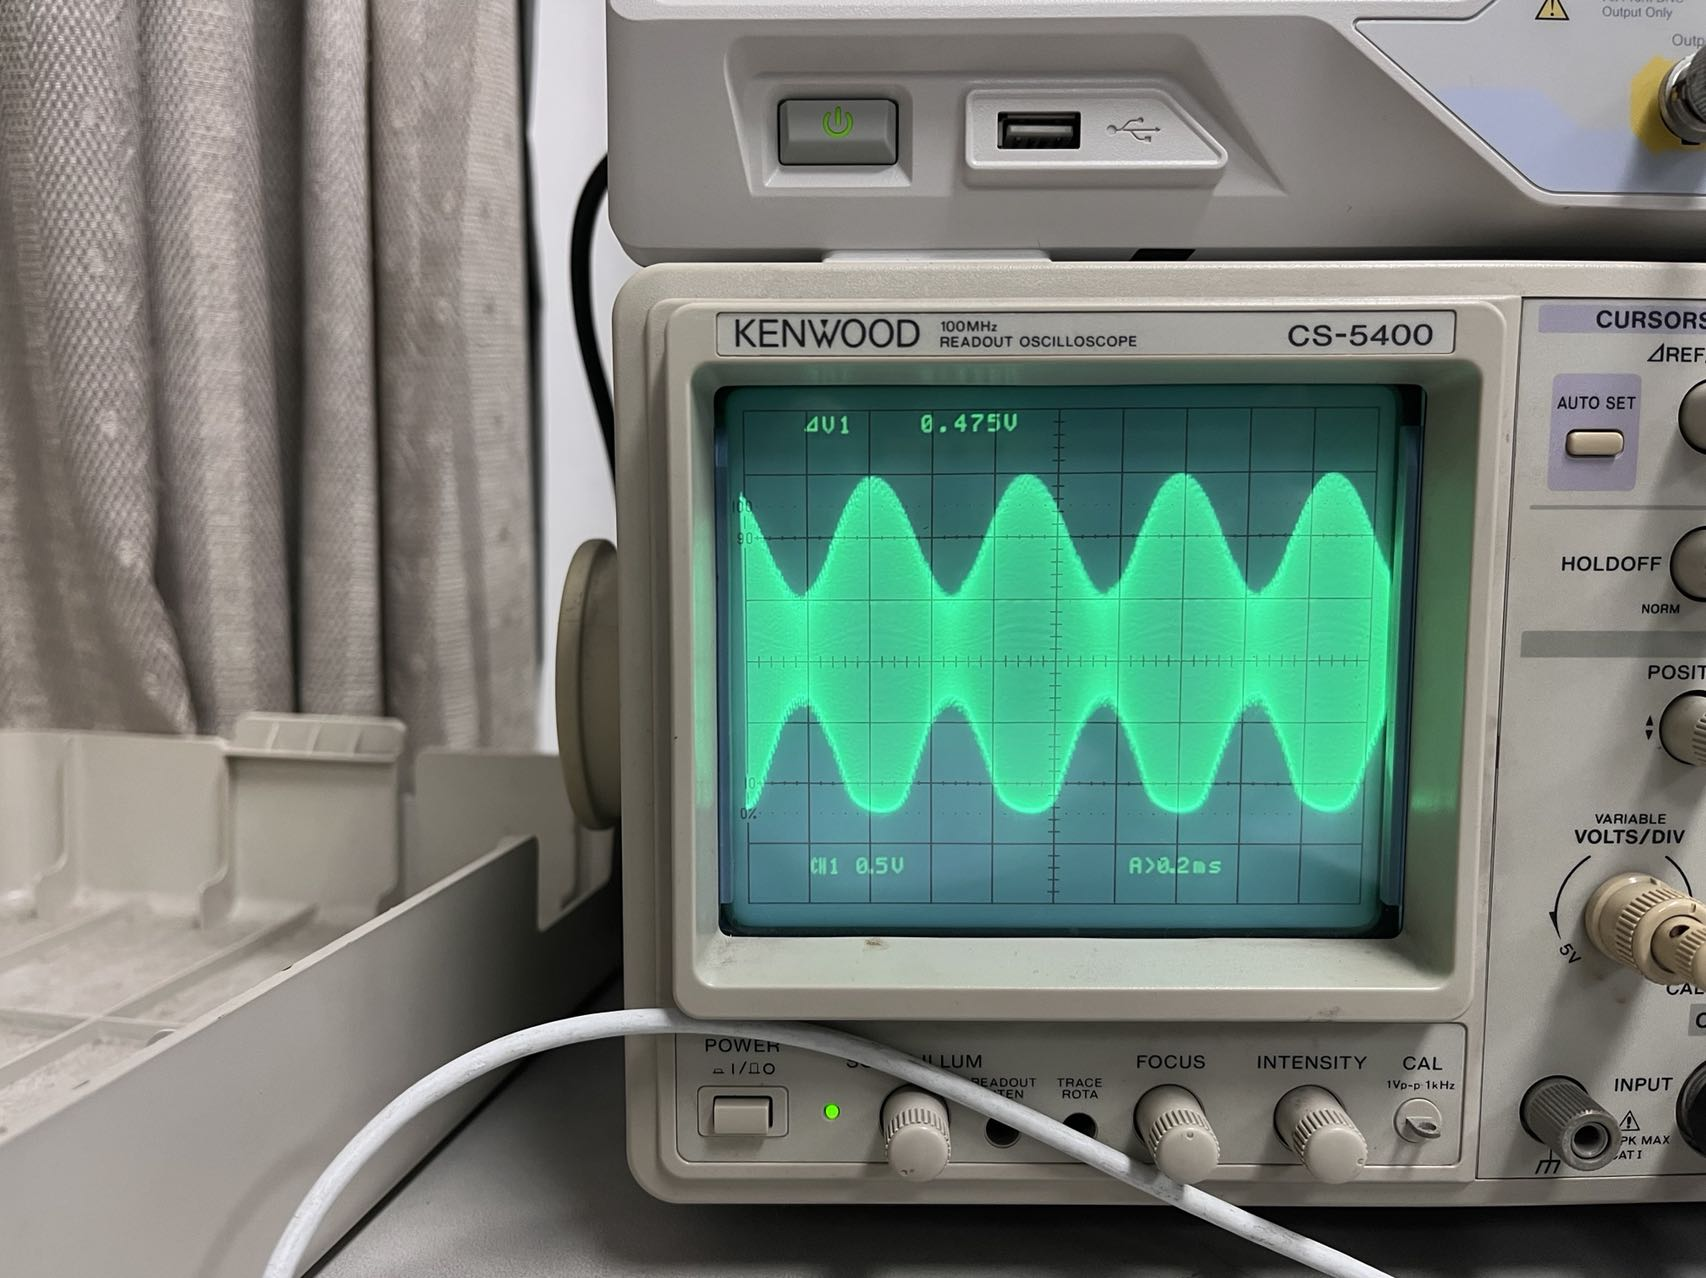
\includegraphics[width = 0.4\textwidth]{7}
                \caption{}
            \end{figure}

            \begin{figure}[H]
                \centering
                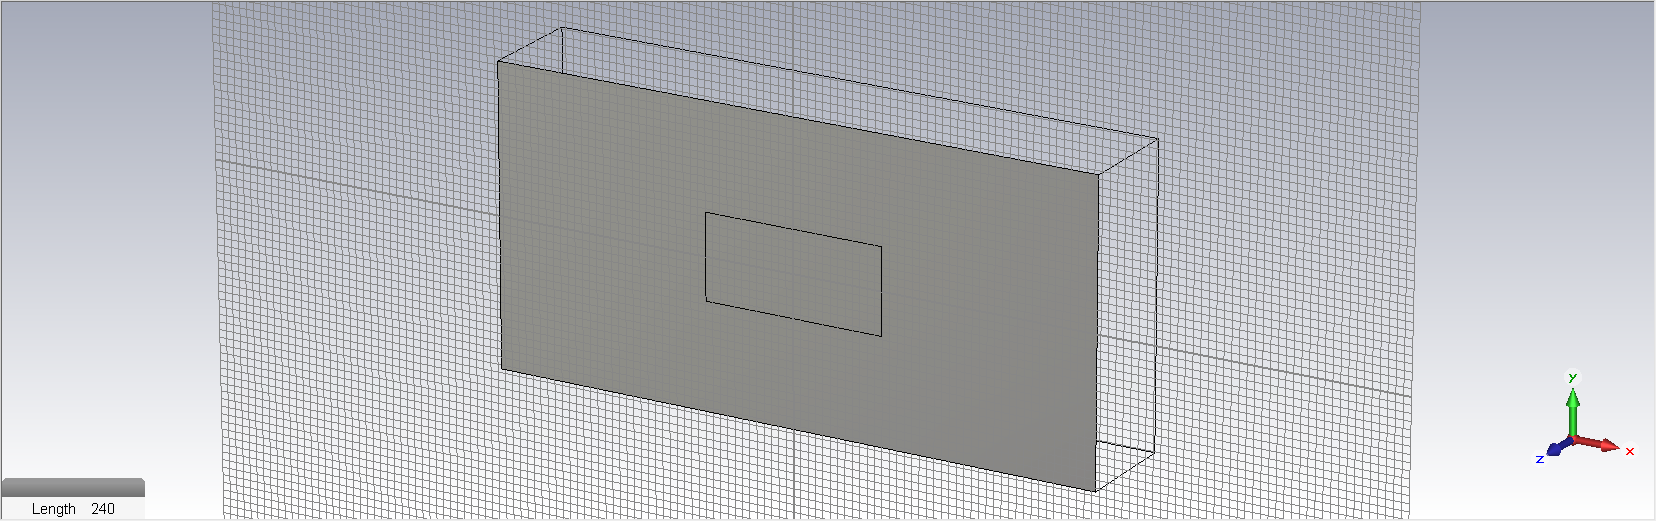
\includegraphics[width = 0.8\textwidth]{8}
                \caption{}
            \end{figure}


            设置喇叭口径面的空间位置

            \begin{figure}[H]
                \centering
                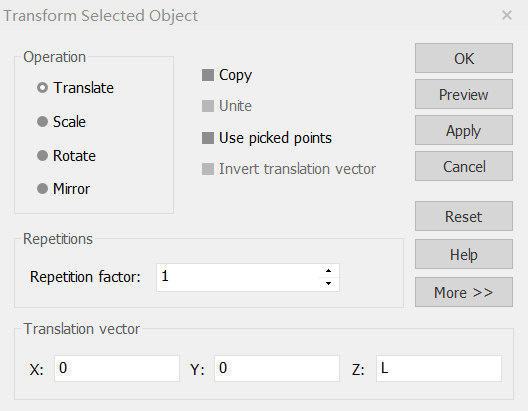
\includegraphics[width = 0.6\textwidth]{9}
                \caption{}
            \end{figure}


            \begin{figure}[H]
                \centering
                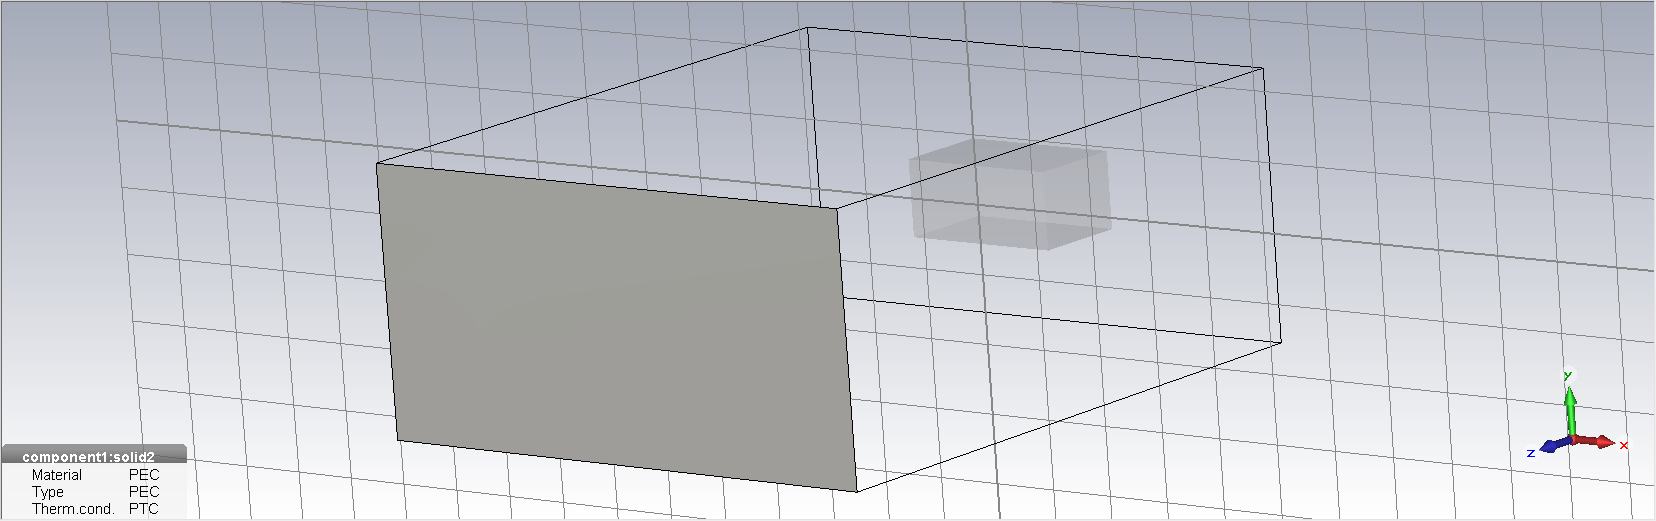
\includegraphics[width = 0.8\textwidth]{10}
                \caption{}
            \end{figure}
            创建喇叭侧壁
            \begin{figure}[H]
                \centering
                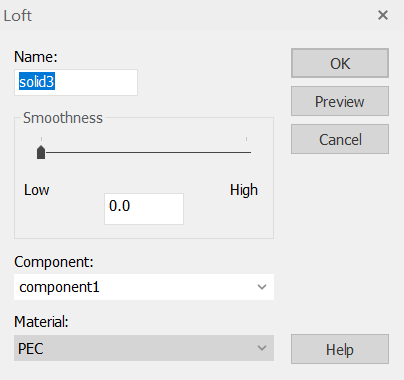
\includegraphics[width = 0.4\textwidth]{11}
                \caption{}
            \end{figure}
            \begin{figure}[H]
                \centering
                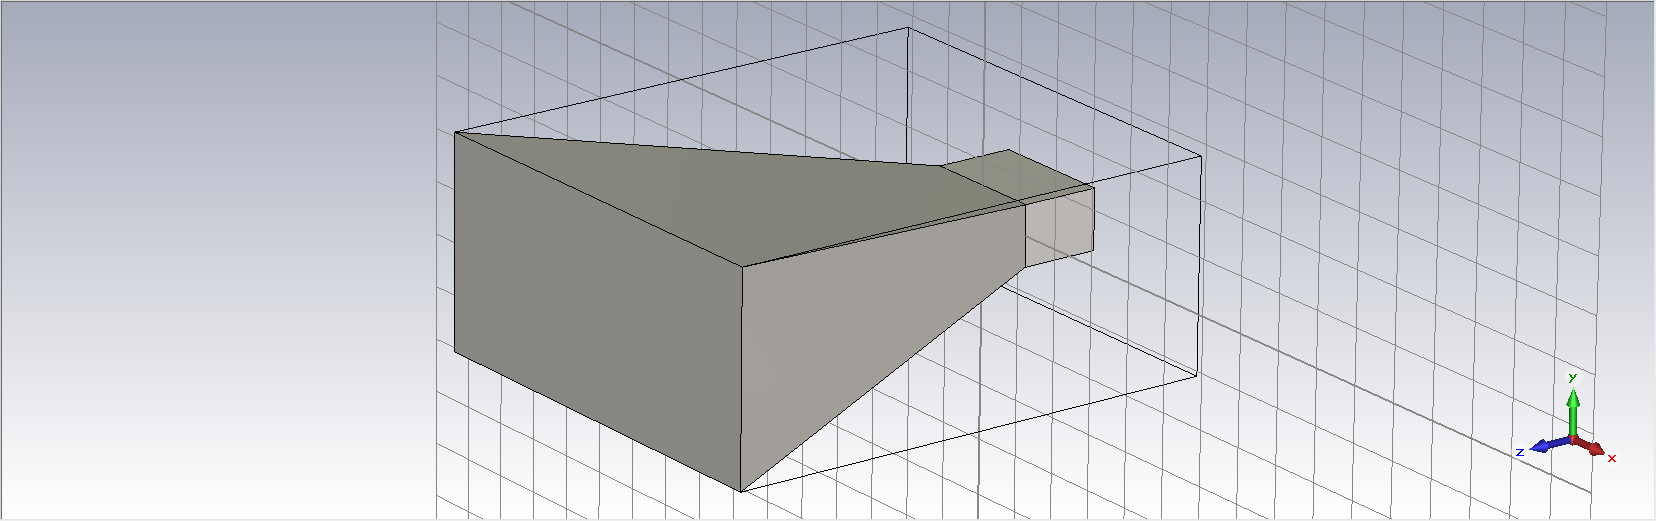
\includegraphics[width = 0.8\textwidth]{12}
                \caption{}
            \end{figure}

            掏空
            \begin{figure}[H]
                \centering
                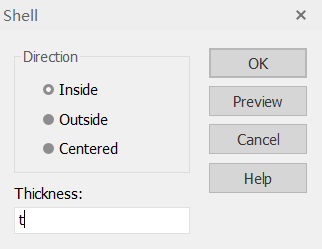
\includegraphics[width = 0.4\textwidth]{13}
                \caption{}
            \end{figure}
            \begin{figure}[H]
                \centering
                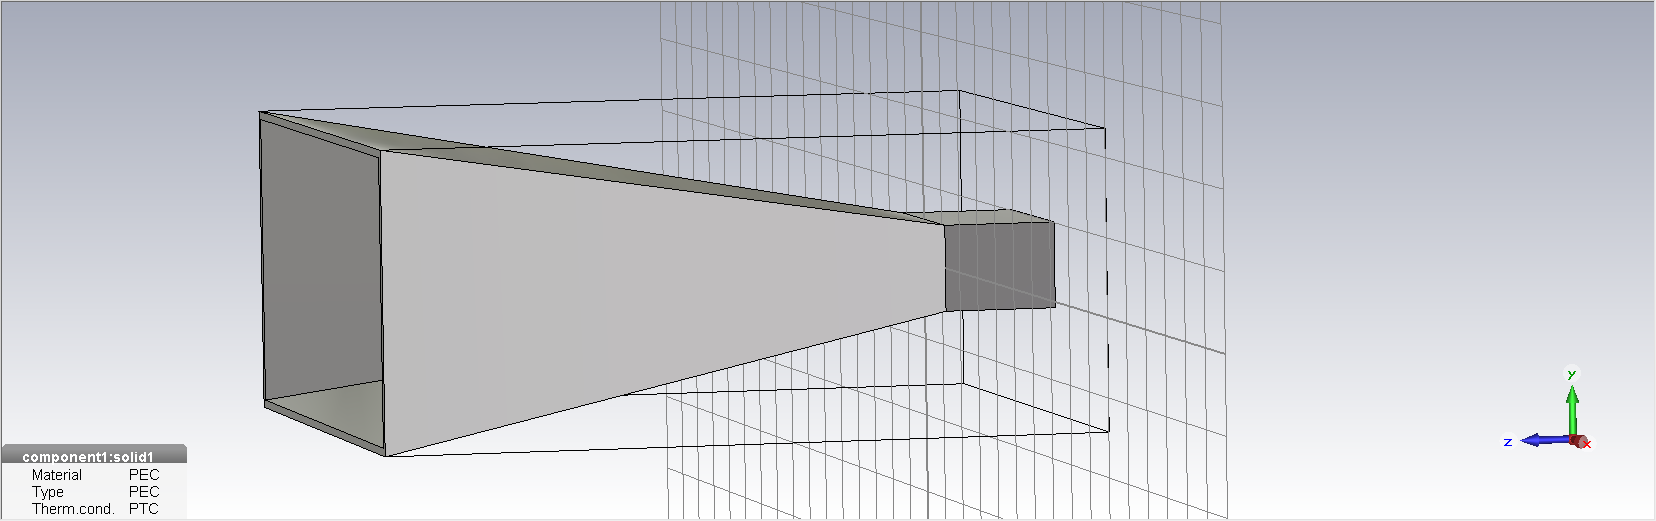
\includegraphics[width = 0.8\textwidth]{14}
                \caption{}
            \end{figure}

        \subsection{仿真分析}

            \subsubsection{仿真条件设置}
            仿真频率
            \begin{figure}[H]
                \centering
                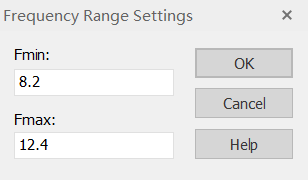
\includegraphics[width = 0.3\textwidth]{15}
                \caption{}
            \end{figure}
            仿真边界条件
            \begin{figure}[H]
                \centering
                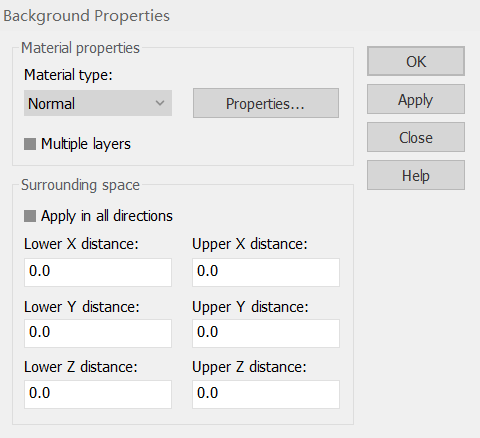
\includegraphics[width = 0.6\textwidth]{16}
                \caption{}
            \end{figure}
            
            \begin{figure}[H]
                \centering
                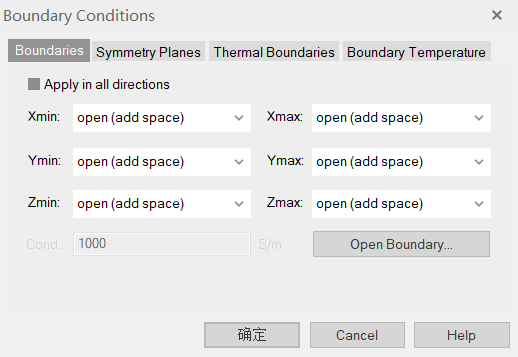
\includegraphics[width = 0.6\textwidth]{17}
                \caption{}
            \end{figure}

            端口设置
            \begin{figure}[H]
                \centering
                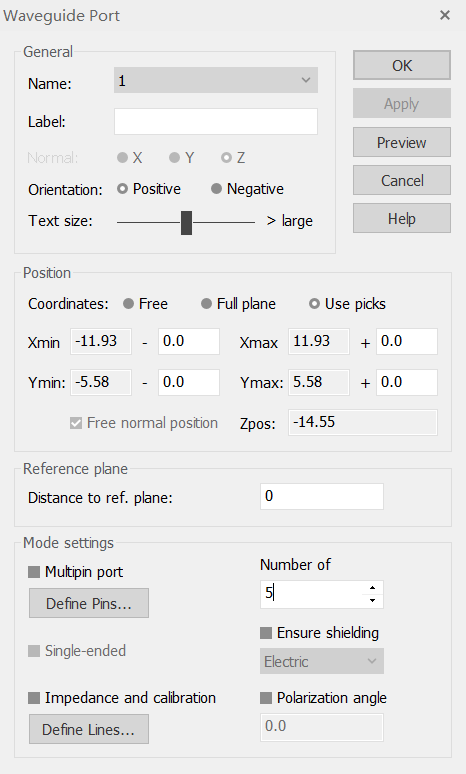
\includegraphics[width = 0.6\textwidth]{18}
                \caption{}
            \end{figure}
            设置监视器
            
            \begin{figure}[H]
                \centering
                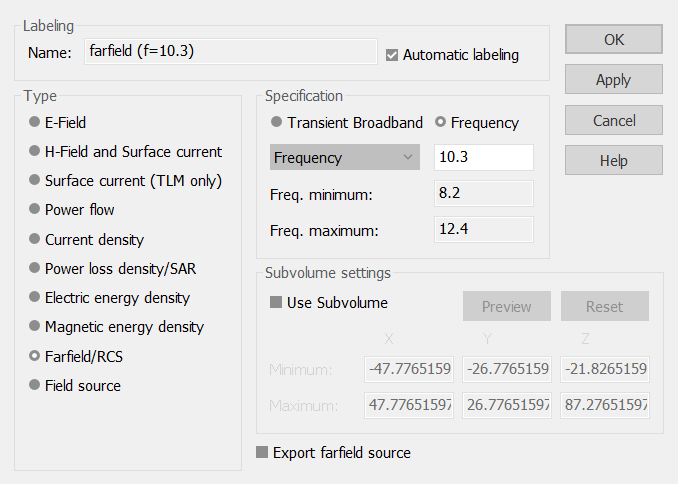
\includegraphics[width = 0.7\textwidth]{20}
                \caption{}
            \end{figure}
            \begin{figure}[H]
                \centering
                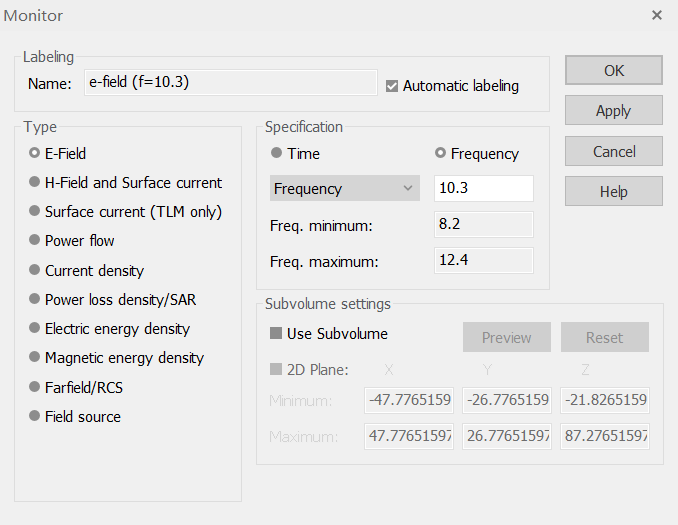
\includegraphics[width = 0.7\textwidth]{24}
                \caption{}
            \end{figure}
            \begin{figure}[H]
                \centering
                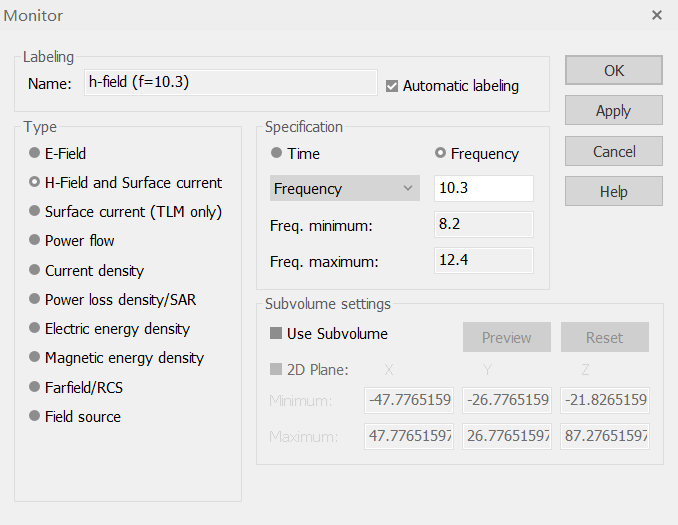
\includegraphics[width = 0.7\textwidth]{25}
                \caption{}
            \end{figure}
            
            \subsubsection{模式分析}
            \begin{figure}[H]
                \centering
                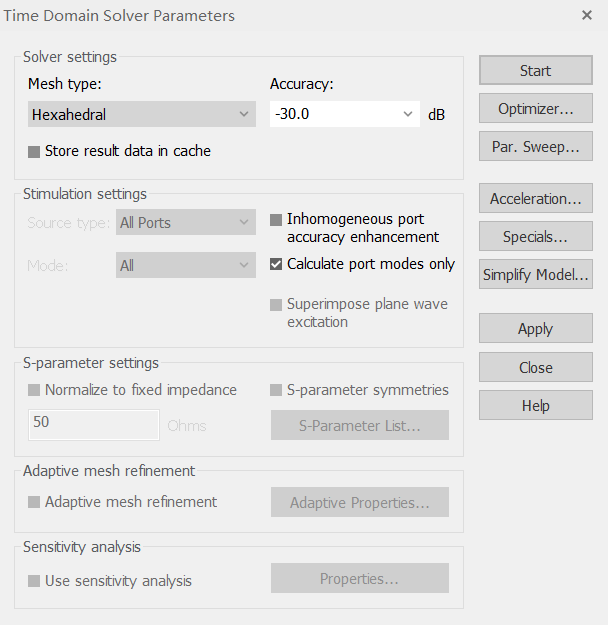
\includegraphics[width = 0.7\textwidth]{21}
                \caption{}
            \end{figure}
            \begin{figure}[H]
                \centering
                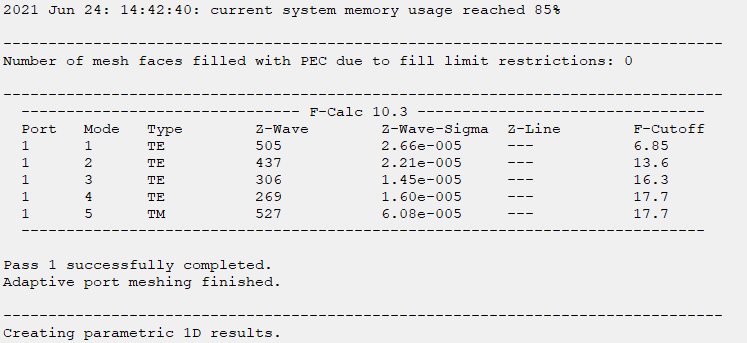
\includegraphics[width = 0.7\textwidth]{22}
                \caption{}
            \end{figure}
            

            由于仿真最高频率为12.4GHz,所以在这种结构的喇叭天线中只传输1 种模式的波,设置的吸收的模式数只要大于1 就可以了。
            \subsubsection{仿真设置}
            \begin{figure}[H]
                \centering
                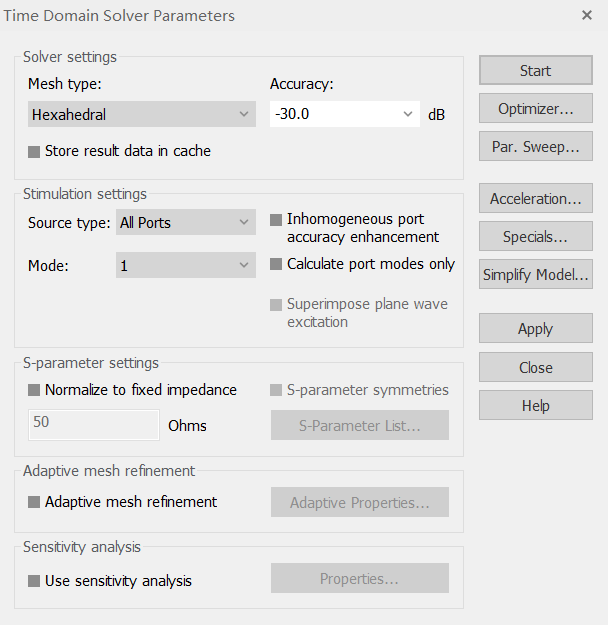
\includegraphics[width = 0.7\textwidth]{23}
                \caption{}
            \end{figure}
            
        \subsection{仿真结果}

            \subsubsection{$S_{11}$曲线}
            \begin{figure}[H]
                \centering
                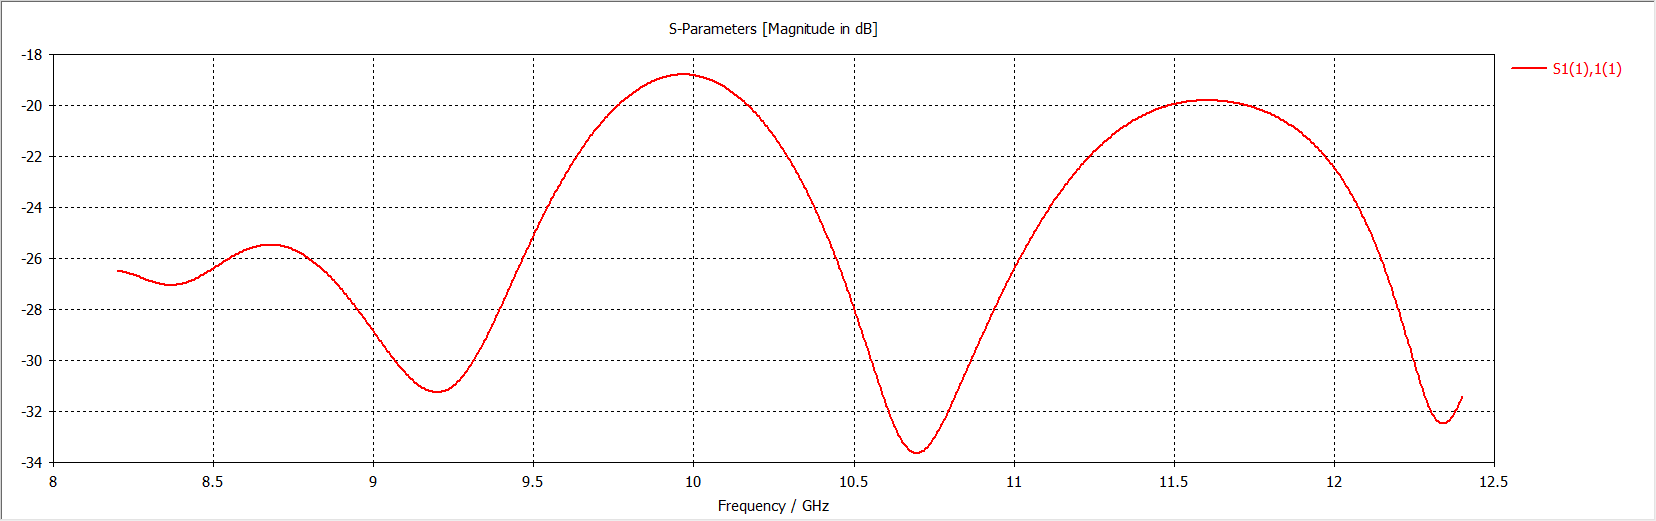
\includegraphics[width = 0.8\textwidth]{S11}
                \caption{}
            \end{figure}
            
            \subsubsection{驻波曲线}
            \begin{figure}[H]
                \centering
                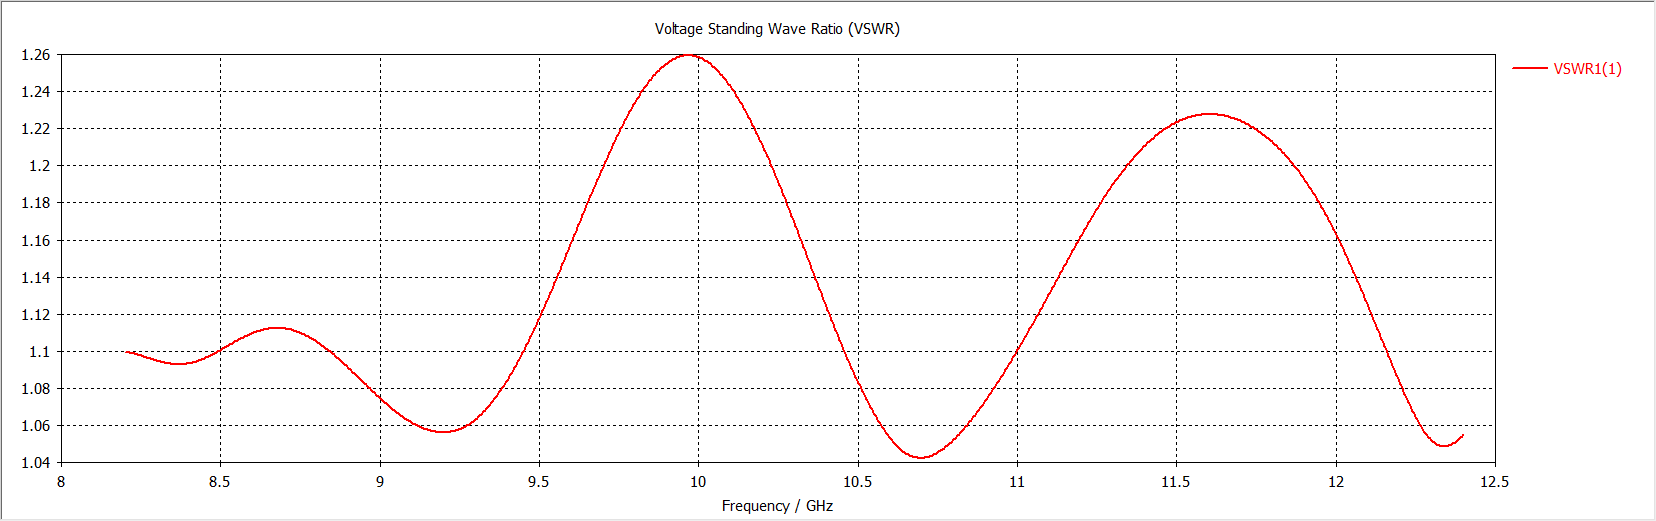
\includegraphics[width = 0.8\textwidth]{VSWR}
                \caption{}
            \end{figure}
            
            \subsubsection{方向图}
            \begin{figure}[H]
                \centering
                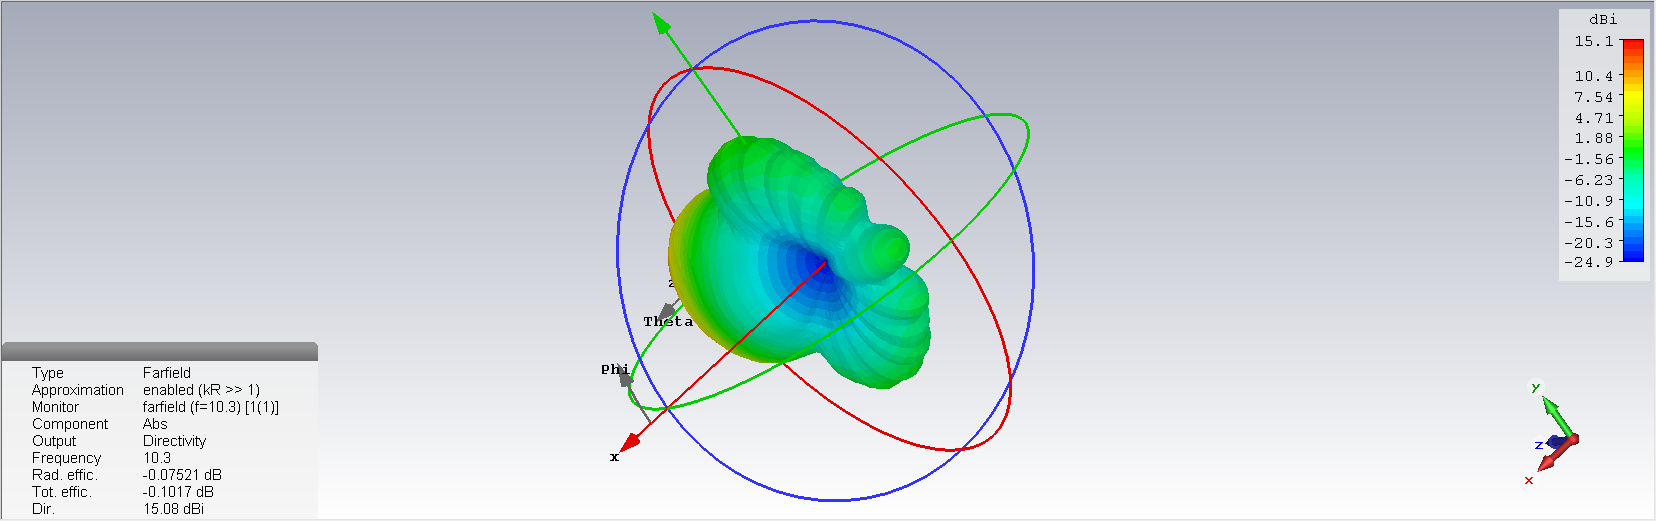
\includegraphics[width = 0.8\textwidth]{Directivity}
                \caption{}
            \end{figure}
            \begin{figure}[H]
                \centering
                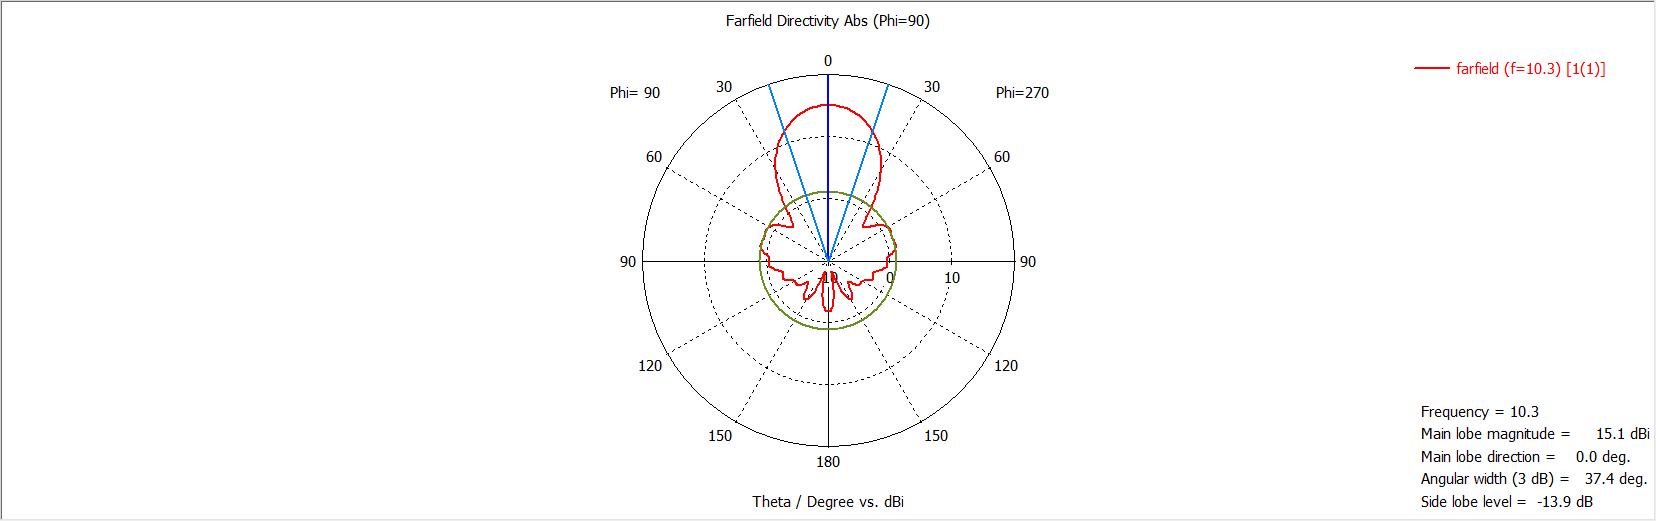
\includegraphics[width = 0.8\textwidth]{Directivity Polar}
                \caption{}
            \end{figure}
            
            \subsubsection{增益图}
            \begin{figure}[H]
                \centering
                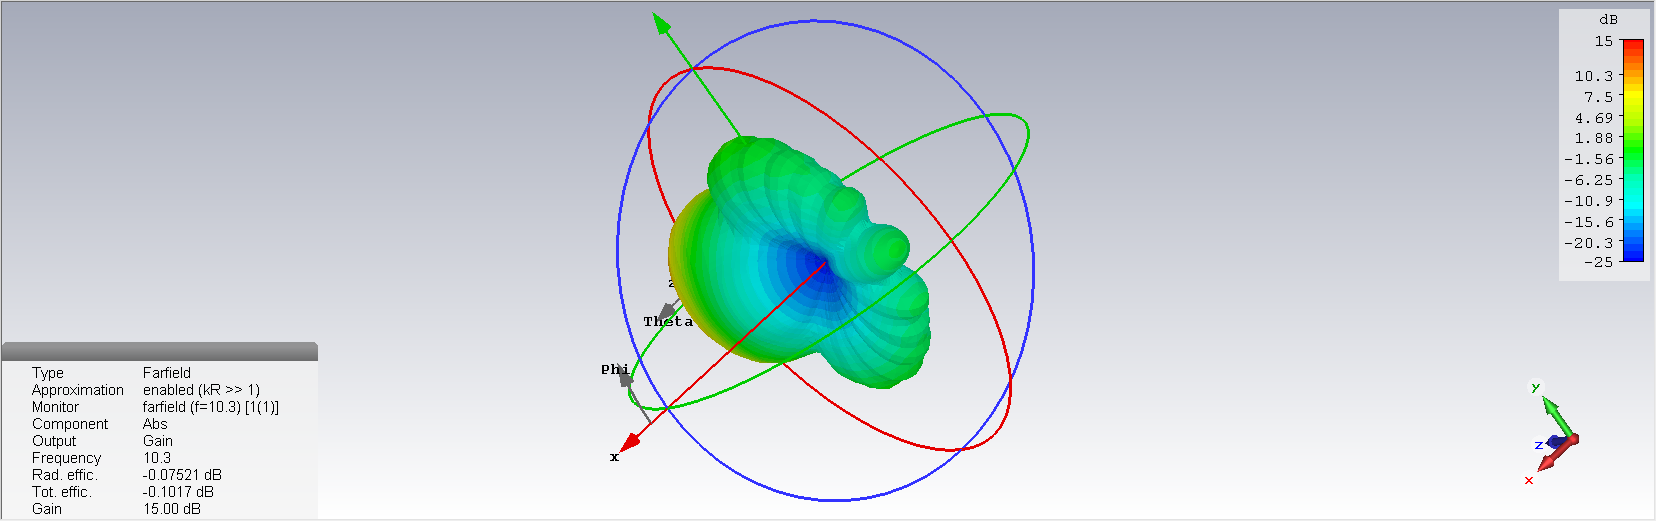
\includegraphics[width = 0.8\textwidth]{Gain}
                \caption{}
            \end{figure}
            \begin{figure}[H]
                \centering
                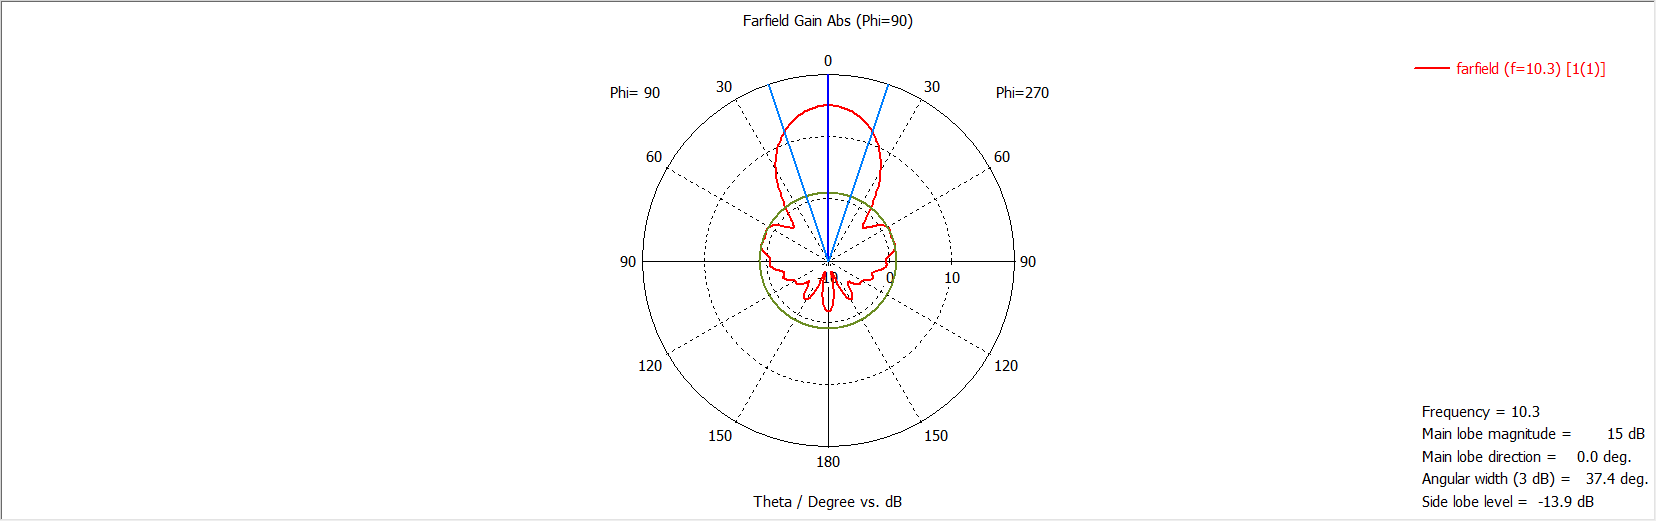
\includegraphics[width = 0.8\textwidth]{Gain polar}
                \caption{}
            \end{figure}
            
            \subsubsection{E-field,  H-field,  surface current图}
            \begin{figure}[H]
                \centering
                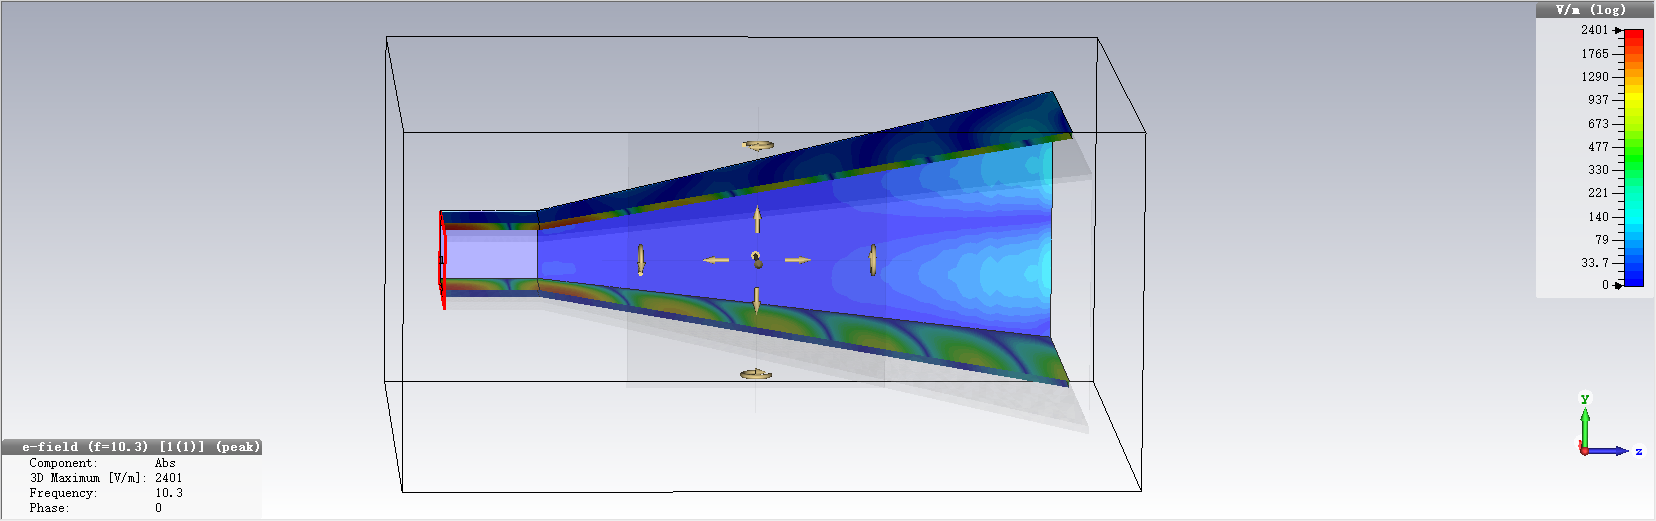
\includegraphics[width = 0.8\textwidth]{e-field}
                \caption{e-field}
            \end{figure}
            \begin{figure}[H]
                \centering
                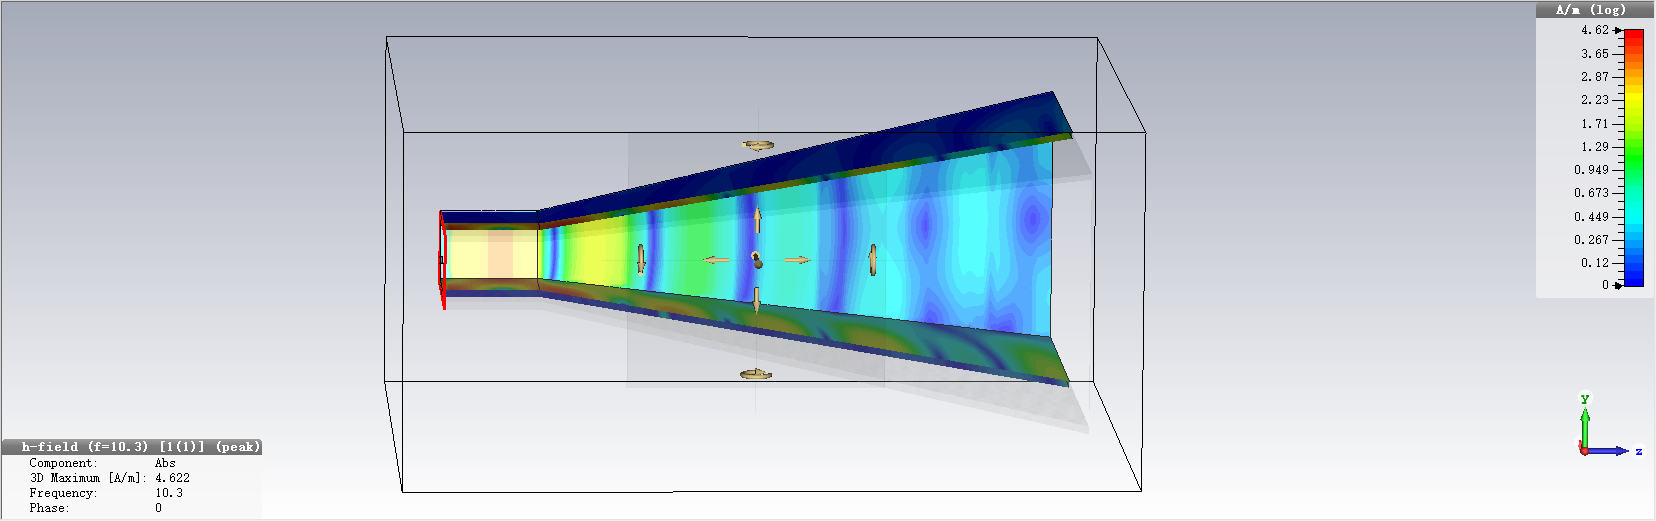
\includegraphics[width = 0.8\textwidth]{h-field}
                \caption{h-field}
            \end{figure}
            \begin{figure}[H]
                \centering
                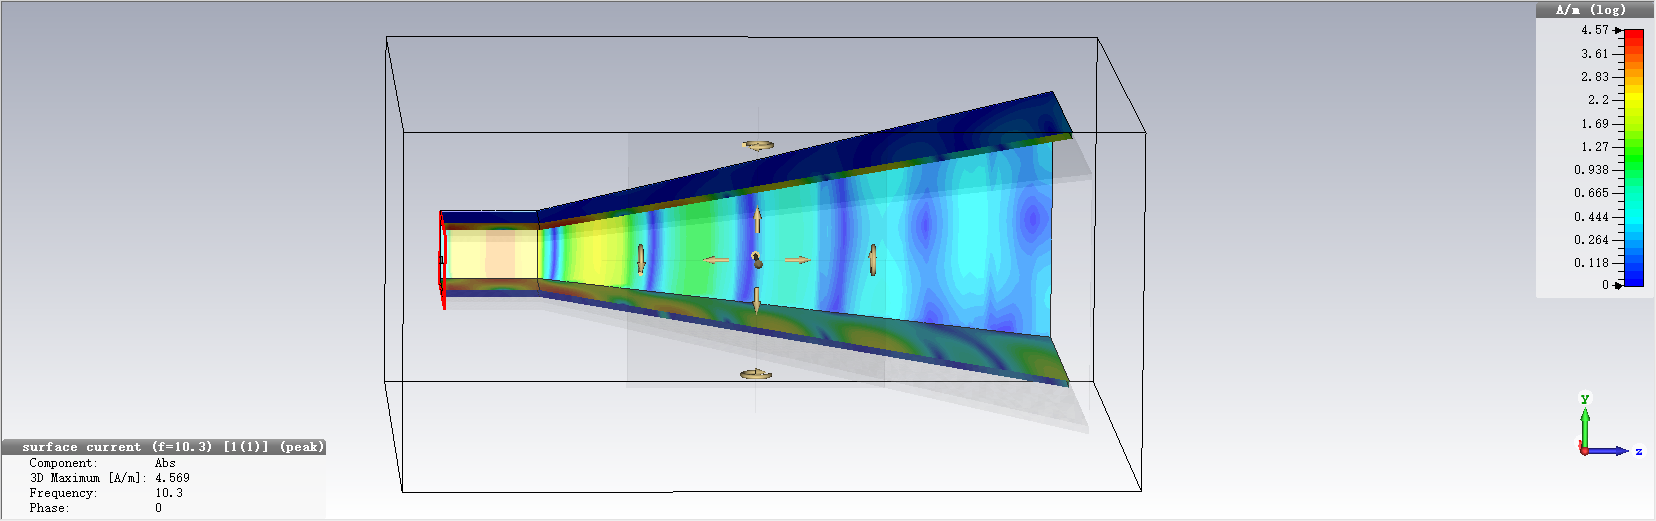
\includegraphics[width = 0.8\textwidth]{surface}
                \caption{surface current}
            \end{figure}
            
        \subsection{分析结论}

            从仿真结果来看,该矩形波导馈电的角锥喇叭天线的主瓣方向为$ \varphi = 0 \deg ,\, \theta = 0 \deg$,主瓣宽度为37.4\degree ,主瓣的最大增益为15dB,最大增益的仿真值与
            理论估计值相近。同时,该天线输入端口的反射系数在工作频段内均在20dB 以下,能够较好的工作。

    \section{实验收获与体会}

    \setcounter{section}{0}
    \setcounter{figure}{0}

    \begin{center}
        \bfseries\Large{喇叭天线的幅射特性测量}
    \end{center}

    \section{实验目的}
        揭示喇叭天线的幅射特性。 \par 
        覆盖的基本概念:
        \begin{itemize}
            \item 天线辐射方向图
            \item 波束宽度
            \item 天线的极化特性
            \item 电磁波在空间传播中与距离的关系
        \end{itemize}
    \section{实验过程与结果}
        \subsection{电磁波在空间传播中与距离的关系测量}
            \begin{table}[H]
                \caption{天线距离与接收功率关系}
                \centering
                \begin{tabular}{|c|c|c|}
                \hline
                距离R(m) & 实验测量值(dB) & 相对归一化数值(dB) \\ \hline
                1      & -40.0     & 0.0         \\ \hline
                1.1    & -41.8     & -1.8        \\ \hline
                1.2    & -43.6     & -3.6        \\ \hline
                1.3    & -45.3     & -5.3        \\ \hline
                1.4    & -46.8     & -6.8        \\ \hline
                \end{tabular}
            \end{table}


        \subsection{极化测量}
            \subsubsection{天线极化测量}
            \begin{table}[H]
                \caption{发射天线喇叭极化特性}
                \centering
                \begin{tabular}{|c|c|c|c|}
                \hline
                发射喇叭天线角度  & 实验测量值(dB) & 相对归一化数值(dB) & 相对归一化功(dB) \\ \hline
                0\degree  & -40.00    & 0.00        & 1.00       \\ \hline
                10\degree & -40.39    & -0.39       & 0.96       \\ \hline
                20\degree & -41.12    & -1.12       & 0.88       \\ \hline
                30\degree & -42.89    & -2.89       & 0.72       \\ \hline
                40\degree & -45.01    & -5.01       & 0.56       \\ \hline
                50\degree & -47.92    & -7.92       & 0.40       \\ \hline
                60\degree & -52.40    & -12.40      & 0.24       \\ \hline
                70\degree & -58.20    & -18.20      & 0.12       \\ \hline
                80\degree & -69.20    & -29.20      & 0.03       \\ \hline
                90\degree & -76.20    & -36.20      & 0.02       \\ \hline
                \end{tabular}
                \end{table}

                


                

                
                
            \subsubsection{极化栅网特性测量}
                \begin{table}[H]
                    \caption{极化栅网极化特性}
                    \centering
                    \begin{tabular}{|c|c|c|c|}
                    \hline
                    极化栅网角度    & 实验测量值(dB) & 相对归一化功率(dB) & 相对归一化功率 \\ \hline
                    0\degree  & -40.0     & 0.0         & 1.00    \\ \hline
                    90\degree & -69.3     & -29.3       & 0.00    \\ \hline
                    45\degree & -44.5     & -4.5        & 0.01    \\ \hline
                    \end{tabular}
                \end{table}
        \subsection{喇叭天线辐射方向图测量}
        \begin{table}[H]
            \caption{天线水平方向图测量数据}
            \centering
            \resizebox{\textwidth}{!}{
                \begin{tabular}{|c|c|c|c|c|c|c|c|c|c|c|c|c|c|c|c|c|c|c|c|}
                    \hline
                    天线水平方向转角(\degree) & -90      & -80      & -70   & -60   & -50   & -40   & -30   & -20   & -10   & 0     & 10    & 20    & 30    & 40    & 50    & 60    & 70    & 80    & 90       \\ \hline
                    实验测量值(dB)         & $\infty$ & $\infty$ & -80.0 & -73.8 & -74.0 & -66.8 & -57.8 & -49.8 & -43.0 & -40.0 & -44.2 & -52.6 & -61.0 & -63.4 & -66.8 & -70.5 & -77.5 & -74.4 & $\infty$ \\ \hline
                    相对归一化数值(dB)       & $\infty$ & $\infty$ & -40.0 & -33.8 & -34.0 & -26.8 & -17.8 & -9.8  & -3.0  & 0.0   & -4.2  & -12.6 & -21.0 & -23.4 & -26.8 & -30.5 & -37.5 & -34.4 & $\infty$ \\ \hline
                    相对归一化功率           & $\infty$ & $\infty$ & 0.01  & 0.02  & 0.02  & 0.05  & 0.13  & 0.32  & 0.71  & 1.00  & 0.62  & 0.23  & 0.09  & 0.07  & 0.05  & 0.03  & 0.01  & 0.02  & $\infty$ \\ \hline
                    \end{tabular}}
            \end{table}

            \begin{table}[H]
                \caption{天线垂直方向测量数据}
                \centering
                \resizebox{\textwidth}{!}{
                    \begin{tabular}{|c|c|c|c|c|c|c|c|c|c|c|c|c|c|}
                        \hline
                        天线垂直方向转角(\degree) & -60   & -50   & -40   & -30   & -20   & -10   & 0     & 10    & 20    & 30    & 40    & 50    & 60    \\ \hline
                        实验测量值(dB)         & -68.6 & -66.2 & -65.5 & -65.2 & -58.6 & -51.5 & -50.0 & -51.5 & -57.2 & -65.0 & -66.0 & -66.2 & -69.0 \\ \hline
                        相对归一化数值(dB)       & -18.6 & -16.2 & -15.5 & -15.2 & -8.6  & -1.5  & 0.0   & -1.5  & -7.2  & -15.0 & -16.0 & -16.2 & -19.0 \\ \hline
                        相对归一化功率           & 0.12  & 0.15  & 0.17  & 0.17  & 0.37  & 0.84  & 1.00  & 0.84  & 0.44  & 0.18  & 0.16  & 0.15  & 0.11  \\ \hline
                        \end{tabular}}
                \end{table}
    \section{实验结果分析}
        \subsection{电磁波传播与距离的关系曲线如下图}

        \begin{figure}[H]
            \centering
            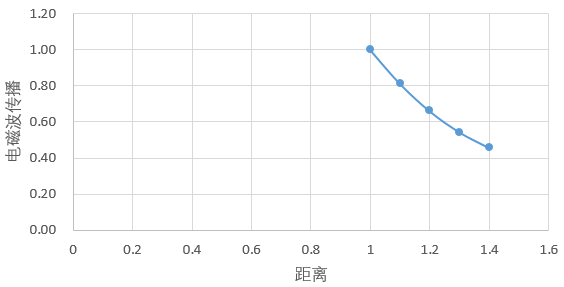
\includegraphics[width = 0.8\textwidth]{pic/电磁波传播与距离的关系曲线.png}
            \caption{电磁波传播与距离的关系曲线}
        \end{figure}

        \subsection{从图中可以看出电磁波传播和距离曲线的关系更接近$1\over R$,由于测得的数据较少,所以不是很明显。}
        
        

        \subsection{发射喇叭天线极化曲线如下图}
        

        \begin{figure}[H]
            \centering
            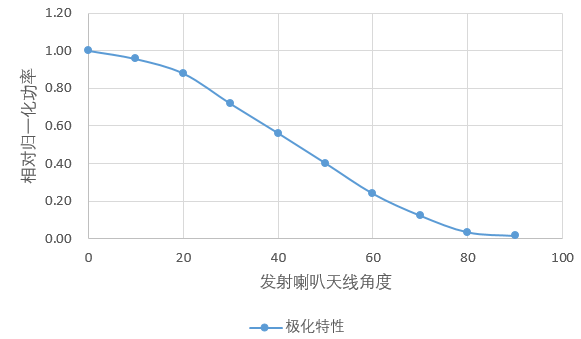
\includegraphics[width = 0.8\textwidth]{pic/发射喇叭天线极化曲线.png}
            \caption{发射喇叭天线极化曲线}
        \end{figure}


        \subsection{问题回答}
            \subsubsection{从下图可以看出,接收喇叭天线所接收到的功率与发射喇叭天线极化角度$\theta$的关系更符合$cos^2 \theta$关系。}

            \begin{figure}[H]
                \centering
                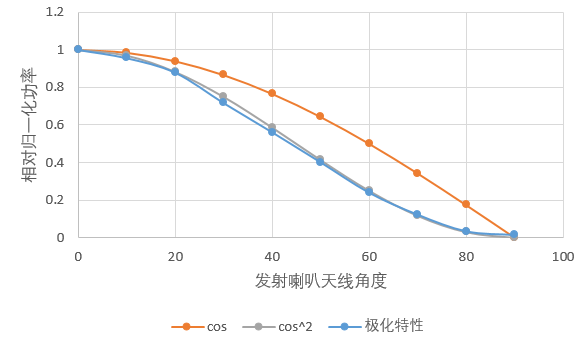
\includegraphics[width = 0.8\textwidth]{pic/发射喇叭天线极化曲线比较.png}
                \caption{发射喇叭天线极化曲线比较}
            \end{figure}

            \subsubsection{发射的信号经过极化器分解成与极化器平行、垂直的两路等幅信号,最终接收喇叭收到一般的信号。
            }

        \subsection{远区场条件}

        实验中:$R = 1.2m, \, D_E = 3.7cm, \, D_H = 8.2cm, \, \displaystyle \frac{2 D_E D_H}{\lambda} = 18.96cm, \,  \therefore   R \gg  \displaystyle \frac{2 D_E D_H}{\lambda} $

        所以符合远区场条件。

        \subsection{理论增益、半功率波束宽度计算}
            \subsubsection{发射喇叭}
            最佳增益:
            
            $\lambda = \displaystyle \frac{c}{f} = 3.2cm$

            $G=0.51 \displaystyle \frac{4 \pi A_{P}}{\lambda^{2}}=0.51 \displaystyle \frac{4 \pi \times 3.7 \times  8.2 }{3.2^{2}}=18.99$

            喇叭天线半功率波束宽度:

            H面:$2 \theta_{0.5} \approx 1.18 \displaystyle \frac{\lambda}{D_{H}}=1.18 \displaystyle \frac{3.2}{8.2}=0.46(\mathrm{rad})$

            E面:$2 \theta_{0.5} \approx 0.89 \displaystyle \frac{\lambda}{D_{E}}=0.89 \displaystyle \frac{3.2}{3.7}=0.77(\mathrm{rad})$

            \subsubsection{接收喇叭}
            最佳增益:
            
            $\lambda = \displaystyle \frac{c}{f} = 3.2cm$

            $G=0.51 \displaystyle \frac{4 \pi A_{P}}{\lambda^{2}}=0.51 \displaystyle \frac{4 \pi \times 10.5 \times  14.1 }{3.2^{2}}=92.66$

            喇叭天线半功率波束宽度:

            H面:$2 \theta_{0.5} \approx 1.18 \displaystyle \frac{\lambda}{D_{H}}=1.18 \displaystyle \frac{3.2}{14.1}=0.27(\mathrm{rad})$

            E面:$2 \theta_{0.5} \approx 0.89 \displaystyle \frac{\lambda}{D_{E}}=0.89 \displaystyle \frac{3.2}{10.5}=0.27(\mathrm{rad})$
            
            结论:喇叭口的面积$A_p$越大,增益越大,斑驳功率波束宽度越小。

        \subsection{方向图}
        
        \begin{figure}[H]
            \centering
            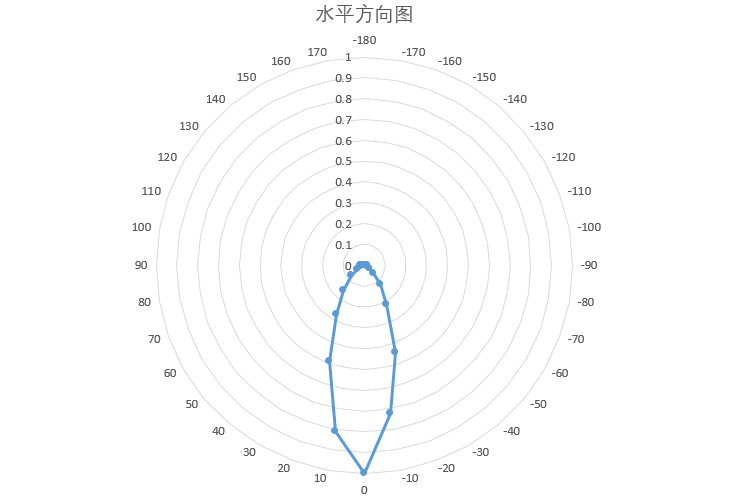
\includegraphics[width = 0.8\textwidth]{pic/水平.png}
            \caption{水平方向图}
        \end{figure}

        \begin{figure}[H]
            \centering
            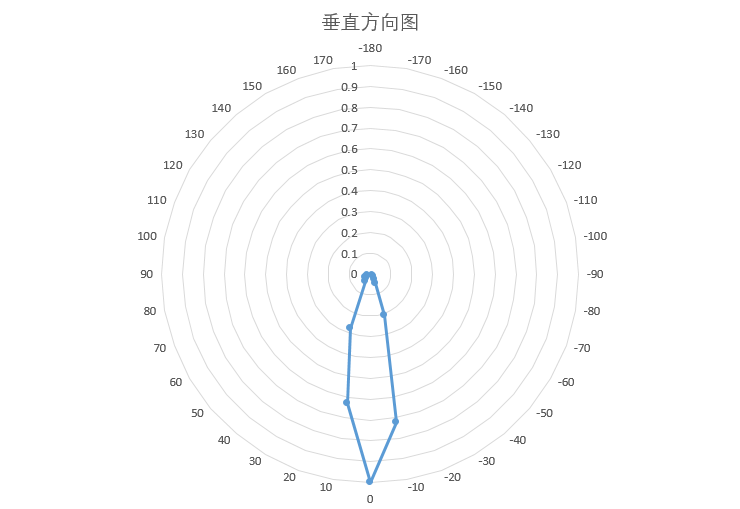
\includegraphics[width = 0.8\textwidth]{pic/垂直.png}
            \caption{垂直方向图}
        \end{figure}


        \subsection{比较半功率波束宽度的计算值与实测值}
        实验测得水平面上波束宽度为29.5\degree ,折合为0.51rad,与计算值0.46rad相比偏大。
        \subsection{ 解释在$\pm 90 \deg$时辐射方向图测量值}
        在$\pm 90 \deg$时测得辐射值并非为零,这是因为存在背景噪声的干扰以及发射的电磁波在四周反射后也会被接收。

    \section{实验收获与体会}
        通过本次实验,我对理论课上学到的有关天线的知识更加熟悉了。同时也通过实验验证电磁场与电磁波的理论。

        实验时我们发现周围环境对实验的干扰很大,所以我们尽量减少走动,以减少实验误差。
\end{document}